\section{Theorie}
\label{sec:Theorie}

% zielsetzung
In diesem Versuch wurden verschieden elektrische Bauteile in Brückenschaltungen
eingesetz, um deren (komplexen) Widerstände zu bestimmen.

Dabei wird hier mit der Nullmethode gearbeitet, d.h. dass durch variable Bauteile
die Brückenspannung zum verschwinden gebracht wird.

\subsection{Kirchoffschen Gesetze}
\label{sec:kirchhoff}
Zur Berechnung vom Stromfluss in Schaltungen werden zwei Gesetze, die
kirchhoffschen Gesetze, verwendet:
\begin{enumerate}
	\item Die \textbf{Knotenregel} besagt, dass an jedem Punkt in einem Stromkreis
		die Summe aller Ströme (wobei Eingangsströme mit $\mathbf{I} > 0$ und
		Ausgangsströme mit $\mathbf{I} < 0$ betrachtet werden) verschwindet:
		\begin{equation}
			\sum_k \mathbf{I}_k = 0.
			\label{eqn:knotenregel}
		\end{equation}
		\begin{figure}[H]
			\centering
			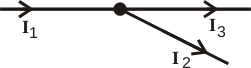
\includegraphics[width=0.4\textwidth]{bilder/knotenregel.png}
			\caption{Darstellung eines ``Knotens`` in einem Stromkreis}
			\label{fig:knotenregel}
		\end{figure}
	\item Nach der \textbf{Maschenregel} ist die Summe der Potentialdifferenzen
		in einem geschlossenen Stromkreis (``Masche``) 0:
		\begin{equation}
			\sum_k U_k = \sum_k \mathbf{I}_k R_k= 0
			\label{eqn:maschenregel}
		\end{equation}
		\begin{figure}[H]
			\centering
			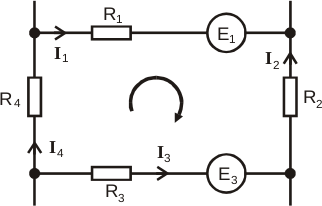
\includegraphics[width=0.5\textwidth]{bilder/maschenregel.png}
			\caption{Darstellung einer Masche in einem Leiternetzwerk}
			\label{fig:maschenregel}
		\end{figure}
\end{enumerate}

\subsection{Berechnung der Brückenspannung und Herleitung der 
Abgleichbedingung}
\label{sec:abgleichbedingung}

In einer Brückenschaltung werden die Stromflüsse in zwei parallelen (jedoch in ihren
Bauteilen nur bedingt gleichen) Stromleitern zwischen zwei Punkten (in 
\autoref{fig:prinzipielle-brueckenschaltung} als A und B bezeichnet) die Potentialdifferenz 
betrachtet.
Diese Potentialdifferenz wird auch im Allgemeinen als Brückenspannung bezeichnet.

\begin{figure}[H]
	\centering
	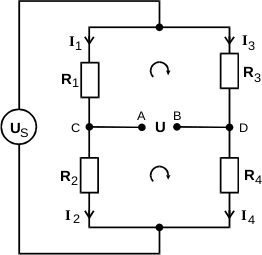
\includegraphics[width=0.5\textwidth]{bilder/prinzipielle-brueckenschaltung.png}
	\caption{Prinzipielle Brückenschaltung}
	\label{fig:prinzipielle-brueckenschaltung}
\end{figure}

Mit dem ersten kirchhoffschen Gesetz lassen sich dann für $U=0$ die Bedingungen für
die parallelen Ströme herleiten:
\begin{equation}
	\mathbf{I}_1 = \mathbf{I}_2
	\quad \text{und} \quad
	\mathbf{I}_3 = \mathbf{I}_4.
	\label{eqn:brueckenschaltung-stroeme}
\end{equation}

%%%% hier noch ne herleitung %%%%%

\autoref{eqn:brueckenspannung-unabhaengig} liefert einen Ausdruck für die Brückenspannung
welche nur von den Widerständen $R_i$, jedoch nicht von der Speisespannung $U_S$ abhängt.
Diese verschwindet, wenn
\begin{equation}
	R_1R_4 = R_2R_3
	\label{eqn:prinzipielle-abgleichbedingung}
\end{equation}
erfüllt ist. Im Falle $U=0$ spricht man auch von einer abgeglichenen Brücke. Da die 
Abgleichbedingung nur von den Widerständen abhängt, kann damit ein unbekannter Widerstand
bestimmt werden. Die Genauigkeit von einer Messung hängt dann nur noch von der Genauigkeit
der bekannten Widerstände und davon, wie niedrig die Brückenspannung in ihrem Minimum ist
(da $U=0$ auch nur ein theoretisches Optimum ist).
Da die Brückenspannung proportional zur Speisespannung ist, sollte diese möglichst
groß gewählt werden.

\subsection{Verallgemeinerung auf komplexe Widerstände}
\label{sec:komplexe-widerstände}
Wenn die Brückenschaltung nicht nur Widerstände, sondern auch Kapazitäten und Induktivitäten
enthält, muss der Formalismus aus \autoref{eqn:abgleichbedingung} auf diese verallgemeinert
werden. Dazu bietet sich die Darstellung als komplexer Widerstand
\begin{equation}
	Z = X + jY
	\label{eqn:komplexer-widerstand}
\end{equation}
an, wobei X den leistungsverbrauchenden Wirkwiderstand und Y den Blindwiderstand darstellt.

Die Abgleichbedingung aus \autoref{eqn:prinzipielle-abgleichbedingung} muss dann als komplexe
Gleichung interpretiert werden, d.h. dass Imaginär- und Realteil auf beiden Seiten gleich sein
müssen. Da aus der Darstellung als komplexer Widerstand zwei Unbekannte ($X$ und $Y$) resultieren,
folgen damit auch zwei Gleichungen:
\begin{equation}
	X_1X_4 - Y_1Y_4 = X_2X_3 - Y_2Y_3 
	\quad \text{und} \quad
	X_1Y_4 - X_4Y_1 = X_2Y_3 - X_3Y_2.
	\label{eqn:komplexe-abgleichbedingung}
\end{equation}
Elektrotechnisch bedeutet dies, dass sowohl Betrag, als auch Phase des Wechselstroms verschwinden
müssen. Aus den zwei Freiheitsgraden folgt auch, dass an der Brückenschaltung zwei voneinander
unabhängige Stellglieder existieren müssen.

\subsection{Verwendete Widerstände}
\label{seq:widerstände}
In diesem Versuch werden ausschließlich Ohm'sche Widerstände benutzt. Von Interesse sind dabei
die Intuktivität (Zeichen: L), die Kapazitäten (C) und die gewöhnlichen, nicht-komplexen 
Widerstände R.

Die Impedanzen im komplexen sind dabei
\begin{align}
	Z_R &= R, \\
	Z_L &= j\omega L, \\
	Z_C &= -\frac{j}{\omega} L. \\
	\label{eqn:impedanzen}
\end{align}
Damit muss beachtet werden, dass diese auch von der Kreisfrequenz des Wechselstroms $\omega$ 
abhängig sein können. 

\subsection{Beschreibung der verwendeten Brückenschaltungen}
\label{sec:spezielle-Schaltungen}

Im Nachfolgenden Abschnitt wird auf einige spezielle Brückenschaltungen eingegangen und mithilfe von
\autoref{eqn:prinzipielle-abgleichbedingung} und \autoref{eqn:komplexe-abgleichbedingung} 
eine Formel für das unbekannte Bauteil hergeleitet.

\subsubsection{Wheatstonesche Brücke}
\label{sec:WheatstonescheBrücke}
In der Wheatstoneschen Brücke sind alle $R_i$ ohmsche Widerstände, wobei hier $R_1$ ein unbekannter
Widerstand ist, die Anderen sind bekannt.

\begin{figure}[H]
	\centering
	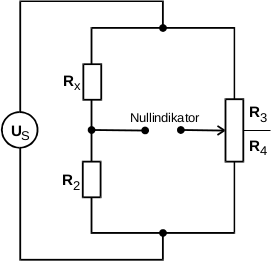
\includegraphics[width=0.4\textwidth]{bilder/wheatstone.png}
	\caption{Schaltplan der Wheatstoneschen Brückenschaltung}
	\label{fig:wheatstone-bruecke}
\end{figure}

Mit \autoref{eqn:prinzipielle-abgleichbedingung} lautet dann der unbekannte Widerstand
\begin{equation}
	R_x = R_2 \frac{R_3}{R_4}.
	\label{eqn:wheatstone-rx}
\end{equation}

\subsubsection{Kapazitätsmessbrücke}
\label{sec:kapazitaetsmessbruecke}

\subsubsection{Induktivitätsmessbrücke}
\label{sec:induktivitätsmessbrücke}

\subsubsection{Maxwell-Brücke}
\label{sec:maxwell-bruecke}

\subsubsection{Wien-Robinson-Brücke}
\label{sec:wien-robinson-bruecke}


\cite{sample}
